\documentclass{article}
\usepackage[pdfborder={0 0 0}, colorlinks=false]{hyperref}
\usepackage{multicol}
\author{CISC475/675 Spring 2010}

% \title{REX User's Manual}
\title{The Hitchhiker's Guide To REX}
\date{\today}

\begin{document}
\maketitle
\tableofcontents
\newpage

\section{Introduction}
The REX software package was designed as part of the CISC475 course,
to create a solution for Prof\. Harvey. Prof\. Harvey wishes to create
multiple versions of each exam for the classes he instructs. However,
this can be very time consuming, and as the number of exams created
increases, the amount of effort needed to be exerted to assure the
accuracy of the exams increases proportionally.

We sought to solve these problems for Prof\. Harvey, and created the
REX software as an educational exercise in real-world software
development practices.

The REX software runs without any installation requirements beyond the
need of an appropriate Java VirtualMachine. The REX software will take
UEF File and an ECF File as input, and non-deterministically save
some number of exam files and answer key files in a desired directory.

\section{Installation}
The REX software does not require any installation. It is suggested to
place the \texttt{rex.jar} executable in a directory within the user
path on UNIX systems, but this is not necessary for proper operation
of the software.

While REX does not require an installer or any unpacking of it's software,
there must be a version of the Java Runtime Environment installed. The
following list of system requirements must be met in order to run REX.

\subsection{Minimum System Requirements}
\begin{itemize}
\item Java Runtime Environment (JRE) 1.6: 

Available at 
\verb|http://java.sun.com/javase/downloads|
% do we need memory requirements? like a 1G of ram? -Haley
\end{itemize}

\section{Usage}
After creating a UEF and ECF file \texttt{rex input.uef input.ecf}. 
REX will parse the contents of the UEF and ECF and generate the
appropriate number of output exams, as specified in the ECF file.

Please see the following sections for information on UEF and ECF
content format.

\section{The UEF File}

Please see Figure \ref{fig:SampleUEF} for an example Universal Exam File.

\section{The ECF File}
The ECF file is a text file with a \texttt{.tex} extension that consists
of a series of constraints. Each constraint is separated by a semicolon,
with comments being all text that follows after a pound symbol 
(\texttt{#}) until the end of the line.

There are four defined commands for the ECF file
\subsection{Group Constraints}
A group constaint is a command of the form \texttt{'include' <integer>
'problems on' <string> 'with difficulty in' <interval> 'at' <integer>
'points' ';'}

\subsection{Required Problem Constraints}

\subsection{Append Text}

\subsection{Version Definition
}

\section{Troubleshooting}
Because of the requirements that REX places upon the input it parses,
REX may present the user with a variety of errors. Additionally, it's
possible that REX might process the request without any errors or warnings,
but will provide an undesired output.

\subsection{Errors}
\subsubsection{RexParseException}
This error means that REX encountered a syntactic error in either the
UEF or ECF file. Please consult the provided error message for more
information.

\subsubsection{RexUnsatisfiableException}
This error means that the input files were parsed correctly, but that
REX determined that the requirements from the ECF cannot be resolved
using the provided UEF file. Generally, this means that there aren't
enough problems in the UEF. Either reduce the number of requested
problems in the ECF, or create new problems in the UEF to resolve
this error.

Note: REX resolves the requirements in the ECF simultaneously. This means
that if the ECF has two identical requirements of 5 questions each, REX
will require at least 10 satisfactory questions.

\section{Credits}
REX was coded by Prof. Siegel's CISC475 class for the 2010 Spring
semester. The TA for this class was Charlie Greenbacker.

\begin{multicols}{2}
\begin{itemize}
\item Aaron Landwehr
\item Ahmed El-Hassany
\item Anthony Platt
\item Burke Cates
\item Fran "Da Man" Fitzpatrick
\item Greg Simons
\item Haley Boyd
\item Ian Burns
\item Jack Song
\item James Cardona
\item Jeremy Verchick
\item Jesse Gledhill
\item Josh Rothhaupt
\item Justin Johnson
\item Keith McLoughlin
\item Kevin Schultz
\item Kyle Bouchard
\item Lucero Carmona
\item Reed Martz
\item Tim Armstrong
\item Tim McClory
\item Trevor Kiernan
\item William Gordon
\item Zach Hine
\end{itemize}
\end{multicols}

% How do we add color to this to make it easier
% to read? -Haley
\begin{figure}
\begin{verbatim}
    \documentclass{exam} 
    \usepackage{fullpage}
    \usepackage{amsmath}
    \usepackage{comment}
    \usepackage{graphicx}

    \begin{document}

    \examheader{CISC 106}{UEF Example}{Developed: 2010}

    \section{Topic}

    \begin{block}{FSA Description}
      In the following four problems, let $A$ denote a finite-state
      automaton with exactly one accepting state.
    \end{block}

    \begin{problem}{topic}{15}
      This is a problem
      \begin{answers}
        \answer This is an answer that is not correct
        \answer answer
        \answer[fixed] This is a fixed answer that is not correct
        \answer[correct] This is a correct answer
        \answer answer
        \answer[fixed,correct] fixed correct answer
      \end{answers}
    \end{problem}

    \begin{figure}[placement h]
      \begin{center}
          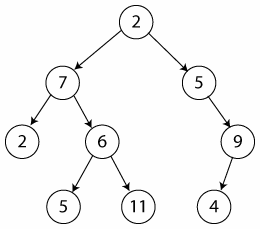
\includegraphics[scale=0.50]{binary_tree.png}
          \caption{Traverse Binary Tree}
          \label{fig:binary tree}
      \end{center}
    \end{figure}

    \begin{block}{Goodbye Message}
      Did you remember to write your name on the first page?  Did you
      attempt to answer every question?    Have a good holiday.
    \end{block}

    \end{document}
\end{verbatim}
\caption{Sample UEF.txt}
\label{fig:SampleUEF}
\end{figure}

\end{document}
